\documentclass[prl,aps,epsf,showpacs,twocolumn,letterpaper]{revtex4}
\usepackage[T1]{fontenc}
\usepackage{newtxtext, newtxmath}
\usepackage{graphicx}
\usepackage{float}
\usepackage{latexsym,amsmath,amssymb,bm,euscript,braket}
\usepackage{color}
\usepackage{subfigure}
\usepackage{epstopdf}
\usepackage[colorlinks=true,linkcolor=blue,citecolor=blue]{hyperref}
\usepackage{hyperref}

%%%%%%%%%%%%%%%%%%%%%%%%%%%%%%%%%%%%%%%%
% FOR MAC'S PERSONAL USE WITH "chktex" %
%%%%%%%%%%%%%%%%%%%%%%%%%%%%%%%%%%%%%%%%
% spaces after commands
% chktex-file 1
% spaces before '('
% chktex-file 36

%%%%%%%%%%%%%%%%%%%%%%%%%%%%%%%%%%%%
% Automatic numbering for sections %
%%%%%%%%%%%%%%%%%%%%%%%%%%%%%%%%%%%%
\let\oldsection\section
\renewcommand{\section}[1]{\stepcounter{section}\oldsection{\Roman{section}. #1}}

%%%%%%%%%%%%%%%%%%%%%%%%%%%%%
% Define the trace operator %
%%%%%%%%%%%%%%%%%%%%%%%%%%%%%
\DeclareMathOperator{\tr}{Tr}

\newcommand{\oim}[1]{{\color{red}$\clubsuit$ #1}}

\bibliographystyle{apsrmp}

\begin{document}



\title{Many-Body Localization in Spin Chain System with a Quasi-Periodic Potential}
\author{Mac Lee, Thomas R. Look, S. P. Lim and D. N. Sheng}

\affiliation{Department of Physics and Astronomy, California State University,
Northridge, California 91330, USA}


\begin{abstract} 


\end{abstract}

\pacs{73.40.Hm, 71.30.+h, 73.20.Jc }
\maketitle


\section{Introduction}

The interplay of random disorder with many-body interactions has attracted a lot of recent research activity\cite{basko2006, oganesyan2007, pal2010, znidaric2008, huse2013, nandkishore2015, altman2015, huse2014, nandkishore2014, pekker_hilbert2014}.  The many-body localized (MBL) quantum phase\cite{nandkishore2015, altman2015, huse2014, nandkishore2014, pekker_hilbert2014} of matter is distinctly different from both Anderson localization in non-interacting systems and the ergodic (thermal) phase for interacting systems with weaker disorder.  The ergodic phase follows the  eigenstate thermalization hypothesis (ETH) which describes how an isolated self-interacting quantum system can thermalize under its own internal dynamics in agreement with quantum statistical mechanics\cite{deutsch1991, srednicki1994, rigol2008}.  A system in the MBL phase, on the other hand, fails to thermalize even for its highly excited eigenstates on any time scale, resulting in new statistics for such systems\cite{basko2006, oganesyan2007, pal2010, znidaric2008, huse2013, nandkishore2015, altman2015, huse2014, nandkishore2014, pekker_hilbert2014}.  Many remarkable properties of the MBL phase have been established\cite{nandkishore2015, altman2015, huse2013, nandkishore2014, oganesyan2007, pal2010, znidaric2008, rigol2008, serbyn2014, kwasigroch2014, yao2014, vasseur2015, huse2014, serbyn2013, ros2015, chandran2014, grover2014, agarwal2015, knap2015, luitz2015, devakul2015, torres2015, canovi2011, cuevas2012, bauer2013, kjall2014, luca2013, iyer2013, pekker_hilbert2014, johri2014, bardarson2012, andraschko2014, laumann2014, hickey2014, nanduri2014, barlev2014, imbrie2014, groverf2014, ponte2015, huang2015, you2015, serbyn2015, singh2015, barlev2015, deng2015, chen2015} based on extensive theoretical studies.  The existence of both the ergodic and MBL phase suggests a dynamic quantum phase transition between them\cite{basko2006, pal2010, oganesyan2007, kjall2014, vosk_theory2014, potter2015trans, serbyn2015, agarwal2015, knap2015, lim2016, zhang2016, zhang2016a, yu2016, vedika2016, dumitrescu2017}.  Random disorder introduces rare Griffiths regions\cite{vosk_theory2014, potter2015trans, knap2015,luitz2015,lim2016} which may have singular contributions in driving such a phase transition, but there is still a limited quantitative understanding of their effects\cite{vedika2017}.  Most numerical studies of the MBL transition have focused on random disorder models for spin chains\cite{pal2010, kjall2014, luitz2015, yu2016, vedika2016}, while very recently the dynamic quantum phase transition has been analyzed with a close comparison between the quasi-periodic and random disorder models, which point to the possibility of two universality classes for the quantum phase transition\cite{vedika2017, vedika2016}.

Time evolution of many-body systems have been studied for spin-chains with a randomly distributed field\cite{kjall2014,luitz2016time}, which can be used to address the dynamics of the thermal to MBL phase transition\cite{nandkishore2015,vosk_theory2014,potter2015}.  After a global quantum quench, power-law growth of bipartite entanglement entropy is observed for thermal states while logarithmic growth is observed for MBL states where a local memory of an initial product state persists for all time\cite{luitz2016time}.

In this paper we report eigenstate and time-dependent studies of spin chains with quasi-periodic disorder.  Through exact diagonalization (ED) and level spacing statistics, we find a dynamic quantum phase transition from the ergodic phase to the MBL phase that is similar to spin chains with random disorder.  However, systems with quasi-periodic disorder appear to be more efficient at localizing which is demonstrated by a smaller critical disorder, $W_c \sim 2$, when compared to systems with random disorder.  We also time-evolve randomly selected product states and study how entanglement entropy and other observables behave as a function of time.  Similar to random field systems, we find that bipartite entanglement entropy in the ETH and MBL phases experience power-law and logarithmic growth, respectively, while the phases are separated by a transition at $W_c$.  Interestingly, we also observe quasi-periodic oscillations of entanglement entropy on short timescales in the MBL phase.  Preservation of imbalance and spin glass order on extremely long timescales for $W > W_c$ are also signatures of the MBL phase.  Our results show that quasi-periodic systems are quantitatively similar to random disorder systems with respect to these standard statistical measurements.


\section{Model and identify the ergodic to many-body localized phase transition}


We study the Heisenberg spin-1/2 chain with a quasi-periodic potential
\begin{equation}
H = J\sum_{i=1}^{N-1} \mathbf{S}_i \cdot \mathbf{S}_{i+1} + \sum_{i}^{N} W\cos(2\pi c i+\phi) S_i^z \text{.}
\end{equation}
where $\mathbf{S}_i$ is the spin operator for site $i$, $J$ is the nearest neighbor coupling constant which we set to $J=1$, $W$ is the quasi-periodic disorder strength, $c$ is an irrational wave number chosen to be $c=\sqrt{2}$, and $\phi$ is a random phase used to create different disorder configurations.  This model is similar to the one studied recently in \cite{vedika2016}.  In this paper, however, we focus on the time-evolution which has not been studied for systems with quasi-periodic potentials.  We use open-boundary conditions which allows for a larger window to observe the time evolution of physical quantities\cite{luitz2016time} before they saturate due to finite-size effects.  All results are obtained for highly excited states near the center of the eigenenergy spectrum.

\begin{figure}
	\includegraphics[angle=-90,width=0.9\linewidth]{entropy_plot.ps}\\	\includegraphics[angle=-90,width=0.9\linewidth]{dispersion_plot.ps}\\ \caption{
		(Color online) For system sizes $L = 10-16$ we notice that both the bipartite entanglement entropy (top) and dispersion (bottom) decay with increasing $W$.  Both graphs display crossing at around $W_c\sim1.6$, indicating a quantum phase transition at that point.  Agreement between these plots supports the conclusion that thermalization fails at high disorder strength.}
	\label{fig1}
\end{figure}

\begin{figure}[b]
	\includegraphics[angle=-90, origin=c, width=3.2in]{newfig1a.ps}\\
	\vspace{-0.6in}
	\includegraphics[angle=-90,width=3.1in]{newfig1b.ps}\\
	\vspace{0.1in}
	\caption{
		(Color online) (a) In this log-log plot, for systems with $W<W_c$ we observe power-law growth of entropy $S(t)$ which saturates at the $L=16$ Page value. (b) Semi-log plot of $S(t)$ with $W > W_c$ indicating logarithimc growth of $S(t)$.}
	\label{fig2}
\end{figure}

\begin{figure*}[t]
	\centering
	\includegraphics[angle=-90,width=2.3in]{newfig1c.ps}
	\includegraphics[angle=-90,width=2.3in]{newfig1d.ps}
	\includegraphics[angle=-90,width=2.3in]{newfig1e.ps}
	\caption{
		(Color online) (a) For system sizes ranging from $12$ to $20$, at $W=1$, we observe that $S(t)$ increases rapidly until $t \sim 1$.  When $1<t<50$, $S(t)$ for all $L$ data fits into a straight line.  For larger $t$, we see that $S(t)$ saturates to $\frac{L}{2} \ln{2}$,  consistent with the thermal entropy of the ergodic phase. (b) At $W=2$, for smaller system sizes, we observe that $S(t)$ grows slower than predicted by the power law; on the other hand, $L=20$ behaves as expected and the growth of its entropy over time follows the power law. (c) At $W=3$, we notice that all $S(t)$ plots fit to a straight line in the semi-log plot, indicating logarithmic growth.}
	\label{fig3}
\end{figure*}


We perform Lanczos ED calculations to obtain energy eigenstates around the energy $E$ at a target energy density $\varepsilon$ for systems with different number of sites $L=10-16$ in the total $S_z=0$ sector.  Specifically, for each disorder configuration, we first calculate the ground state energy $E_0$ and the maximum energy $E_\text{max}$, which are used to define the target energy density $\varepsilon = (E-E_0)/(E_\text{max} -E_0)$.
%Physical quantities\cite{luitz2015}  including the bipartite entanglement
%entropy,  energy level statistics and bipartite  fluctuation of the subsystem
%magnetization are obtained and averaged over disorder configurations and
%sometimes also averaged over  30 energy eigenstates with energies closest to
%the given energy density $\varepsilon$ as detailed below.
We first locate the critical point for the MBL phase transition based on the entanglement entropy and the fluctuations of the half-system magnetization\cite{luitz2015}.  The Von Neumann entanglement entropy of a system partitioned down the middle with reduced density matrix $\rho_A$ is given by $S=- \tr (\rho_A \ln \rho_A)$.  We average the bipartite entanglement entropy over 30 ($L=12$) to 200 ($L=16$) eigenstates near target energy $E$ characterized by energy density $\varepsilon=0.5$ using the shift-invert method, and over $1000$ disorder configurations by choosing random $\phi$ between $(0, 2\pi)$.  As shown in Fig. 1(a), we plot the ratio of entanglement entropy over the number of system sites $S/L$ for different systems at energy density $\varepsilon=0.5$ from $L=10$ to $16$ as a function of quasi-periodic field strength $W$.  As $W\to0$ we see $S/L$ increase with $L$ which approaches the Page value ($S/L \sim 0.5\ln(2)$ for large $L$ limit) following the volume law of the ergodic phase.  For larger $W$, $S/L$ approaches zero indicating area law entanglement and non-ergodic behavior where the MBL state is realized.  With varying $W$, all data points approximately cross each other around a critical value $W_c \sim 1.6$.  We compare the entanglement entropy behavior with the bipartite fluctuations $F$ of the subsystem magnetization $S^z_A$~\cite{luitz2015,song2012}, which is defined as $F=\braket{{S^{z}_A}^2} - \braket{S^z_A}^2$ as shown in Fig. 1(b).  We see that $F/N$ increases on the small $W$ side, while it becomes vanishing small on the larger $W$ side.  The $F/N$ curves for different $N$ approximately cross each other around the critical field strength $W_c\sim1.6$, consistent with the behavior of the entanglement entropy.  In fact, we see that there is an approximately proportional relationship between $S$ and $F$  for all $W$ region. 

We then use the level statistics analysis from random matrix theory\cite{atas2013,oganesyan2007} to probe the localization-delocalization characteristics of the energy eigenstates.  
%In the delocalized  regime, the level-spacing  distribution is described by the
%Gaussian orthogonal ensemble (GOE) statistics, which represents extended levels
%with level-repulsion  between them because of the overlap of  energy
%eigenstates in real space.  In the localized regime, the level-spacing
%distribution  is determined by Poisson statistics as  wave-functions close in
%energy are exponentially localized with no level repulsion between
%them\cite{mehta1991}.
In energy spectrum analysis\cite{luitz2015}, we define the adjacent energy gap $\delta_n=E_n-E_{n-1}$ as the energy difference between the $n$-th and $(n-1)$-th eigenstates, then the adjacent gap ratio can be defined as $r_n=\min(\delta_n, \delta_{n+1})/\max(\delta_n, \delta_{n+1})$.  We average the gap ratio $r=\langle r_n\rangle$ over $30-200$ states near the spectrum center at $\varepsilon=0.5$ and more than 1000 random potential configurations for each given disorder strength $W$.  As shown in Fig. 1(c), we see that at the small $W$ side, $r$ approaches the Gaussian orthogonal ensemble value ($0.5307$), which represents extended levels with level-repulsion between them because of the overlap of energy eigenstates in real space.  On the stronger $W$ side, $r$ reaches the Poisson value $(2\ln2-1\simeq 0.3863)$ for larger systems representing the level statistics of localized states, where states close in energies are exponentially localized with exponential small overlap without level repulsion between them\cite{mehta1991}.  A similar level crossing for all curves is also seen in Fig.1(c), indicating the same critical point for the dynamic quantum phase transition.  We also note that, the critical point we determined represents a lower bound for the transition as the crossing points between larger $L$ curves move towards the larger $W$ side.  This feature was also observed in a different model for quasi-periodic systems\cite{vedika2016}.


\subsection{Time-Evolution of quantum state}


We study the quantum dynamics of the quasi-periodic systems after a global quantum quench.  Here we start from a product state $\ket{\Psi(0)}=\ket{\sigma_1, \sigma_2, \ldots , \sigma_L}$  at the time $t=0$ after the quench, where $\sigma_i=\pm$ represents the spin-z component $\pm 1/2$ at site $i$.  The state at time $t$ can be obtained as $\ket{\Psi(t)} = e^{-iHt}\ket{\psi(0)}=e^{-iH\Delta t}\ket{\psi(t-\Delta t)}$ (with setting $\hbar=1$).  We calculate the time evolution of an initial  state  based on  a projection of the Hamiltonian to the Krylov space spanned by $\ket{\Psi_0}$, $H\ket{i\Psi_0}$, \ldots, $H^n\ket{\Psi_0}$ using the Lanczos algorithm by calculating all eigenstates in this space to obtain the time-evolution operator\cite{luitz2015}.  Using a reasonably small time step $\delta t \sim 0.2/J$ allows for highly accurate results with even with small $n=30-60$.

We first discuss the general behavior of the entanglement entropy as a function of time as shown in Fig. 2.  On the small $W$ side shown in Fig. 2(a), we find that the entropy $S(t)$ exhibits power-law growth in time $t$ before it reaches the saturated value $\frac L 2 \ln2$ at long time limit.  On the larger $W$ side, we find a much slower growth, which can be fit with a logarithmic growth function as shown in Fig. 2(b) for $W=3-5$.  

We now analyze the finite-size scaling behavior of $S(t)$.  For small $W=1$ as shown in Fig. 3(a), we find that the initial growth ($t\sim 1$) of $S(t)$ is exponential and system size independent.  For the intermediate time regime, $S(t)$ experiences power-law growth until the finite-size effect sets in.  With the increase of $L$, we find a wider time interval for the power-law growth of $S(t)$.  Interestingly, we see very similar behavior and a smaller window for power-law growth of $S(t)$ for $W=2$.  The power-law growth indicated by the straight line in the Fig.3(b) is most clear for larger system size $L=20$.  This is a strong indication that the $W=2$  is in the thermal phase consistent with the moving of the crossing point toward larger $W$ with the increase of $L$ observed in Fig. 1.  We then look into $S(t)$ at $W=3$ where we observe that for small $t$, $S(t)$ grows exponentially from the product state to a superposition state for $t\sim 1$, which is then followed by oscillations of $S(t)$.  With further increase of $t$, we observe a logarithmic growth of $S(t)$ for a time range of more than two orders of magnitude.  The range of $t$ for logarithmic growth of $S(t)$ becomes larger with the increase of $W$.  These results confirm an MBL phase with similar behavior to the random field case studied by Luitz et. al\cite{luitz2015}. 

Now we address the time evolution of spin correlations.  We start from the product state $|\Psi(0)>$ where the $\sigma_z$ on each site is $\pm 1/2$ while the total $S_z$ of all sites are zero.  We define the following time correlator for $\sigma_z$ as 
\begin{equation}
I(t)=\frac{4}{L} \sum_{j=1}^L \braket{\Psi(0)|S_j^z(0)S_j^z(t)|\Psi(0)} \text{,} \label{eq:imb}
\end{equation}
which detects the total imbalance of $\sigma_z$.  As shown in Fig.4(a), we find a systematic change of the properties of $I(t)$ as $W$ is varied.  For smaller $W=1$, we see that the long time behavior of imbalance $I(t)$ is dominated by  power-law decay $1/t^{\alpha}$, and at the large $t$ limit $\sigma_z$ on a site becomes uncorrelated with the initial condition and $I(t)$ approaches zero.  For intermediate $W=1.5$ and $2$, a similar power-law behavior is obtained with a much smaller decay power $\alpha$, indicating the longer time scale required to approach equilibrium spin correlations for these thermal states near the transition point to the MBL phase.  On the MBL side with $W=3$ and $4$, we see that the $I(t)$ is near constant at large $t$ limit with a near vanishing decay exponent ($\alpha \sim 0$).

\begin{figure}[h]
	\includegraphics[angle=-90,width=3.in]{newfig2a.ps}\\
	\vspace{-0.0in}
	\includegraphics[angle=-90,width=3.in]{newfig2b.ps}\\
	\hspace{0.0in}
	\vspace{-0.in}
	\caption{
		(Color online) (a) Imbalance $I(t)$ for a $L=16$ system with $1 < W < 4$.  At small values of $W$, we notice the imbalance of the system decays rapidly; however, when $W$ is increased beyond $W_c = 1.6$, we notice the imbalance ceases decaying and remains at a certain level.  This is consistent with the MBL behavior where the initial values of the local observables for each site $i$ is preserved. (b) Spin glass order as defined in eq.\ref{eq:sgo}. At small values of $W$, correlations between spins are short ranged and $\chi(t)$ decays to $1$ over time; at large values of $W$, $\chi(t)$ remains close to its initial value even at very long time, further corroborating our assertion of a quantum phase transition.}
	\label{fig4}
\end{figure}

For comparison, we also study spin glass order for the MBL phase.  The spin-flip from the Heisenberg term will create domain walls.  If the domain walls are confined together, a spin-glass order can develop.  We define the spin glass order parameter 
\begin{equation}
\chi^{SG}=\frac 1 L \sum_{i,j=1}^L \braket{\Psi(t)|S_i^zS_j^z|\Psi(t)}^2 \text{,} \label{eq:sgo}
\end{equation}
which can diverge with $L$ in the spin-glass ordered phase.  As shown in Fig.4(b), we see very similar to $I(t)$.  For smaller $W=1-2$, we see that $\chi(t)$ decreases with $t$ in power-law fashion, while it maintains a large value in the long time limit for larger $W>2$.  Our results indicate a jump of the spin glass order at the thermal to MBL transition.  In Fig.5, we see that both $I(t)$ and $\chi(t)$ show very weak size dependence at $W=3$.  Clearly, the spin glass order parameter separates and remains split for different system size for the whole time range, which fully establishes the robustness of the MBL phase.  

\begin{figure}[h]
	\includegraphics[angle=-90,width=0.92\linewidth]{newfig3a.ps}\\ \includegraphics[angle=-90,width=0.92\linewidth]{newfig3b.ps}\\
	\caption{
		(Color online) (a) \bf Needs to be written}
	\label{fig5}
\end{figure} 

\subsection{Summary and Discussions}
                                 

{\bf Acknowledgments} --- The first two authors contributed equally to this
work.  This work is supported by US National Science Foundation  Grants PREM
DMR-1205734 and DMR-1408560.


%%%%%%%%%%%%%%%%%%%%%%%%%%%%%%%%%%%% References
\bibliographystyle{apsrev}
\bibliography{quasi_mbl}


\end{document} 

